\begin{center}
    {\large \textbf{PHẦN I. LÝ THUYẾT XÁC SUẤT}}\\[0.3em]
    {\normalsize \textit{(Probability Theory)}}\\[1em]
    {\LARGE \textbf{CHƯƠNG 2. BIẾN NGẪU NHIÊN}}
\end{center}

\vspace{1em}
\hrule
\vspace{1.5em}

\section{Biến ngẫu nhiên và hàm mật độ}

\subsection{Khái niệm biến ngẫu nhiên}
Xét một phép thử với không gian mẫu $\Omega$.

Giả sử, ứng với mỗi biến cố sơ cấp $\omega \in \Omega$, ta liên kết với một số thực $X(\omega) \in \mathbb{R}$, thì $X$ được gọi là một biến ngẫu nhiên (đại lượng ngẫu nhiên).

Tổng quát, biến ngẫu nhiên (BNN) $X$ của một phép thử với không gian mẫu $\Omega$ là một ánh xạ:
\begin{align*}
X: \Omega &\to \mathbb{R} \\
\omega &\mapsto X(\omega) = x.
\end{align*}
Giá trị $x$ được gọi là một giá trị của biến ngẫu nhiên $X$.

\begin{vidu}
Người A mua một loại bảo hiểm tai nạn trong 1 năm với phí là 70 ngàn đồng. Nếu bị tai nạn thì công ty sẽ chi trả 3 triệu đồng. Gọi $X$ là số tiền người A có được sau 1 năm mua bảo hiểm này. Khi đó, ta có:
\begin{itemize}
    \item Phép thử là: ``mua bảo hiểm tai nạn''.
    \item Biến cố là $T$: ``người A bị tai nạn''.
    \item Không gian mẫu là $\Omega = \{T, \overline{T}\}$.
\end{itemize}
Vậy $X(T) = 2{,}93$ (triệu), $X(\overline{T}) = -0{,}07$ (triệu).
\end{vidu}

\begin{itemize}
    \item Ký hiệu $\{X = x\}$ là một biến cố bao gồm các biến cố sơ cấp $\omega$ sao cho $X(\omega) = x$, nghĩa là:
    \[
    \{X = x\} = \{\omega \in \Omega : X(\omega) = x\}.
    \]
    Tương tự, ta có:
    \begin{align*}
    \{X \le x\} &= \{\omega \in \Omega : X(\omega) \le x\}, \\
    \{X < x\} &= \{\omega \in \Omega : X(\omega) < x\}, \dots
    \end{align*}
\end{itemize}

\begin{vidu}
Tung một đồng xu 2 lần, ta có không gian mẫu:
\[
\Omega = \{NN, NS, SN, SS\}.
\]
Nếu gọi $X$ là ĐLNN thể hiện số lần mặt ngửa xuất hiện, thì:
\[
X(NN) = 2, \quad X(NS) = X(SN) = 1, \quad X(SS) = 0.
\]
\begin{itemize}
    \item Miền giá trị của ĐLNN $X$: $X(\Omega) = \{0, 1, 2\}$.
    \item Xác suất:
    \begin{align*}
    \{X = 0\} &= \{SS\} \Rightarrow P(X = 0) = 1/4, \\
    \{X = 1\} &= \{NS, SN\} \Rightarrow P(X = 1) = 1/2, \\
    \{X \le 1\} &= \{NS, SN, SS\} \Rightarrow P(X \le 1) = 3/4.
    \end{align*}
\end{itemize}
\end{vidu}

\begin{itemize}
    \item Nếu $X(\Omega)$ là 1 tập hữu hạn $\{x_1, x_2, \dots, x_n\}$ hay vô hạn đếm được thì $X$ được gọi là \textbf{biến ngẫu nhiên rời rạc}. Để cho gọn, ta viết là $X = \{x_1, x_2, \dots, x_n, \dots\}$.
    \item Nếu $X(\Omega)$ là 1 khoảng của $\mathbb{R}$ (hay cả $\mathbb{R}$) thì $X$ được gọi là \textbf{biến ngẫu nhiên liên tục}.
    \item Cho biến ngẫu nhiên $X$ và hàm số $y = \varphi(x)$. Khi đó, biến ngẫu nhiên $Y = \varphi(X)$ được gọi là \textbf{hàm của biến ngẫu nhiên} $X$.
\end{itemize}

\subsection{Hàm mật độ}

\subsubsection{Biến ngẫu nhiên rời rạc}
Ta định nghĩa:
\begin{itemize}
    \item \textbf{Bảng phân phối xác suất} của $X$ là:
    \begin{center}
    \begin{tabular}{|c|c|c|c|c|c|}
    \hline
    $X$ & $x_1$ & $x_2$ & \dots & $x_n$ & \dots \\
    \hline
    $P$ & $p_1$ & $p_2$ & \dots & $p_n$ & \dots \\
    \hline
    \end{tabular}
    \end{center}

    \item \textbf{Hàm mật độ} của $X$ là:
    \[
    f(x) = \begin{cases}
    p_i & \text{khi } x = x_i, \\
    0 & \text{khi } x \ne x_i, \forall i.
    \end{cases}
    \]
\end{itemize}

\begin{chuy}
\begin{itemize}
    \item $p_i \ge 0$; $\sum p_i = 1$, $i = 1, 2, \dots$
    \item Nếu $x \notin \{x_1, x_2, \dots, x_n, \dots\}$ thì $P(X = x) = 0$.
    \item $P(a < X \le b) = \displaystyle\sum_{a < x_i \le b} p_i$.
\end{itemize}
\end{chuy}

\begin{vidu}[VD 2]
Cho BNN rời rạc $X$ có bảng phân phối xác suất:
\begin{center}
\begin{tabular}{|c|c|c|c|c|c|}
\hline
$X$ & $-1$ & $0$ & $1$ & $3$ & $5$ \\
\hline
$P$ & $3a$ & $a$ & $0{,}1$ & $2a$ & $0{,}3$ \\
\hline
\end{tabular}
\end{center}
\begin{enumerate}[label=\arabic*)]
    \item Tìm $a$ và tính $P(-1 < X \le 3)$.
    \item Lập bảng phân phối xác suất của hàm $Y = X^2$.
\end{enumerate}

\paragraph{Giải.}
\begin{enumerate}[label=\arabic*)]
    \item Ta có:
    \[
    \sum p_i = 1 \Rightarrow 3a + a + 0{,}1 + 2a + 0{,}3 = 1 \Rightarrow a = 0{,}1.
    \]
    Vậy:
    \begin{align*}
    P(-1 < X \le 3) &= P(X = 0) + P(X = 1) + P(X = 3) \\
    &= 0{,}1 + 0{,}1 + 0{,}2 = 0{,}4.
    \end{align*}
    \item Bảng phân phối xác suất của hàm $Y = X^2$:
    \begin{center}
    \begin{tabular}{|c|c|c|c|c|c|}
    \hline
    $Y$ & $1$ & $0$ & $1$ & $9$ & $25$ \\
    \hline
    $P$ & $0{,}3$ & $0{,}1$ & $0{,}1$ & $0{,}2$ & $0{,}3$ \\
    \hline
    \end{tabular}
    \end{center}
    Thu gọn các giá trị trùng nhau, ta được:
    \begin{center}
    \begin{tabular}{|c|c|c|c|c|}
    \hline
    $Y$ & $0$ & $1$ & $9$ & $25$ \\
    \hline
    $P$ & $0{,}1$ & $0{,}4$ & $0{,}2$ & $0{,}3$ \\
    \hline
    \end{tabular}
    \end{center}
\end{enumerate}
\end{vidu}

\begin{vidu}[VD 4]
Một hộp có 3 viên phấn trắng và 2 viên phấn đỏ. Một người lấy ngẫu nhiên mỗi lần 1 viên (không trả lại) từ hộp đó ra cho đến khi lấy được 2 viên phấn đỏ. Gọi $X$ là số lần người đó lấy phấn. Hãy lập bảng phân phối xác suất và hàm mật độ của $X$?

\paragraph{Giải.} Ta có: $X = \{2; 3; 4; 5\}$.

Gọi $A_i$: ``viên phấn được lấy lần thứ $i$ là đỏ'', $i = \overline{1; 5}$.
Ta có:
\begin{itemize}
    \item $P(X = 2) = P(A_1 A_2) = P(A_1) P(A_2 | A_1) = \dfrac{2}{5} \cdot \dfrac{1}{4} = 0{,}1$.
    \item $P(X = 3) = P(A_1 \overline{A}_2 A_3) + P(\overline{A}_1 A_2 A_3) = \dfrac{2}{5} \cdot \dfrac{3}{4} \cdot \dfrac{1}{3} + \dfrac{3}{5} \cdot \dfrac{2}{4} \cdot \dfrac{1}{3} = 0{,}2$.
    \item $P(X = 4) = P(A_1 \overline{A}_2 \overline{A}_3 A_4) + P(\overline{A}_1 A_2 \overline{A}_3 A_4) + P(\overline{A}_1 \overline{A}_2 A_3 A_4) = 0{,}3$.
    \item $P(X = 5) = 1 - \dfrac{1}{10} - \dfrac{2}{10} - \dfrac{3}{10} = 0{,}4$.
\end{itemize}

Vậy bảng phân phối xác suất của $X$ là:
\begin{center}
\begin{tabular}{|c|c|c|c|c|}
\hline
$X$ & $2$ & $3$ & $4$ & $5$ \\
\hline
$P$ & $0{,}1$ & $0{,}2$ & $0{,}3$ & $0{,}4$ \\
\hline
\end{tabular}
\end{center}

Hàm mật độ của $X$ là:
\[
f(x) = \begin{cases}
0{,}1 & \text{khi } x = 2, \\
0{,}2 & \text{khi } x = 3, \\
0{,}3 & \text{khi } x = 4, \\
0{,}4 & \text{khi } x = 5, \\
0 & \text{khi } x \ne 2, 3, 4, 5.
\end{cases}
\]
\end{vidu}

\subsubsection{Biến ngẫu nhiên liên tục}
Hàm số $f: \mathbb{R} \to \mathbb{R}$ được gọi là \textbf{hàm mật độ} của biến ngẫu nhiên liên tục $X$ nếu:
\[
P(a \le X \le b) = \int_a^b f(x)\,dx, \quad \forall a, b \in \mathbb{R}.
\]

\begin{chuy}
$f(x)$ là hàm mật độ của biến ngẫu nhiên liên tục $X$ khi và chỉ khi:
\[
f(x) \ge 0, \quad \forall x \in \mathbb{R} \quad \text{và} \quad \int_{-\infty}^{+\infty} f(x)\,dx = 1.
\]
\end{chuy}

\begin{nhanxet}
\begin{itemize}
    \item Khi $f(x)$ liên tục trên lân cận của điểm $a$, ta có:
    \[
    P(a - \varepsilon \le X \le a + \varepsilon) = \int_{a-\varepsilon}^{a+\varepsilon} f(x)\,dx \implies P(X = a) = \lim_{\varepsilon \to 0} \int_{a-\varepsilon}^{a+\varepsilon} f(x)\,dx = 0.
    \]
    Vậy:
    \[
    P(a \le X < b) = P(a < X \le b) = P(a < X < b) = \int_a^b f(x)\,dx.
    \]
    \item \textbf{Ý nghĩa hình học:} Xác suất của biến ngẫu nhiên $X$ nhận giá trị trong $[a; b]$ bằng diện tích hình thang cong giới hạn bởi $x = a$, $x = b$, $y = f(x)$ và $Ox$:
    \[
    P(a \le X \le b) = \int_a^b f(x)\,dx = S.
    \]
    \begin{center}
    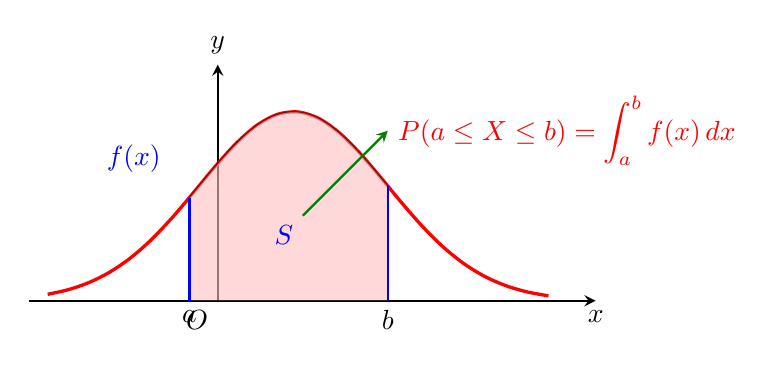
\begin{tikzpicture}[scale=1.2]
        \draw[->, >=stealth, thick] (-2,0) -- (4,0) node[below] {$x$};
        \draw[->, >=stealth, thick] (0,0) -- (0,2.5) node[above] {$y$};
        \node[below left] at (0,0) {$O$};
        
        % Curve
        \draw[domain=-1.8:3.5, smooth, variable=\x, red, very thick] 
            plot ({\x}, {2*exp(-0.5*(\x-0.8)*(\x-0.8))});
        \node[blue, left] at (-0.5,1.5) {$f(x)$};
        
        % Shaded region
        \draw[fill=pink, opacity=0.6] 
            (-0.3,0) -- plot[domain=-0.3:1.8, smooth, variable=\x] ({\x}, {2*exp(-0.5*(\x-0.8)*(\x-0.8))}) -- (1.8,0) -- cycle;
            
        \draw[blue, thick] (-0.3,0) -- (-0.3,{2*exp(-0.5*(-0.3-0.8)*(-0.3-0.8))});
        \draw[blue, thick] (1.8,0) -- (1.8,{2*exp(-0.5*(1.8-0.8)*(1.8-0.8))});
        
        \node[below] at (-0.3,0) {$a$};
        \node[below] at (1.8,0) {$b$};
        \node[blue] at (0.7,0.7) {$S$};
        \draw[->, >=stealth, thick, color=green!50!black] (0.9,0.9) -- (1.8,1.8) node[right, color=red] {$P(a \le X \le b) = \displaystyle\int_a^b f(x)\,dx$};
    \end{tikzpicture}
    \end{center}
\end{itemize}
\end{nhanxet}

\begin{vidu}[VD 5]
Chứng tỏ $f(x) = \begin{cases} 4x^3, & x \in [0; 1] \\ 0, & x \notin [0; 1] \end{cases}$ là hàm mật độ của biến ngẫu nhiên $X$ và tính $P(0{,}5 \le X < 3)$?

\paragraph{Giải.}
\begin{itemize}
    \item Ta có $f(x) \ge 0, \forall x \in \mathbb{R}$ và:
    \[
    \int_{-\infty}^{+\infty} f(x)\,dx = \int_{-\infty}^0 f(x)\,dx + \int_0^1 f(x)\,dx + \int_1^{+\infty} f(x)\,dx = \int_0^1 4x^3\,dx = \left.x^4\right|_0^1 = 1.
    \]
    Vậy $f(x)$ là hàm mật độ của BNN $X$.
    \item Ta có:
    \[
    P(0{,}5 \le X < 3) = \int_{0{,}5}^3 f(x)\,dx = \int_{0{,}5}^1 f(x)\,dx + \int_1^3 f(x)\,dx = \int_{0{,}5}^1 4x^3\,dx = \left.x^4\right|_{0{,}5}^1 = \frac{15}{16}.
    \]
\end{itemize}
\end{vidu}

\begin{vidu}[VD 6]
Cho biến ngẫu nhiên $X$ có hàm mật độ:
\[
f(x) = \begin{cases}
0, & x < 2 \\
\dfrac{k}{x^2}, & x \ge 2.
\end{cases}
\]
Tính $P(-3 < X < 5)$?

\paragraph{Giải.} Do $f(x)$ là hàm mật độ của $X$, nên:
\[
\int_{-\infty}^{+\infty} f(x)\,dx = 1 \Rightarrow k \int_2^{+\infty} \frac{dx}{x^2} = 1 \Rightarrow \left.-\frac{k}{x}\right|_2^{+\infty} = 1 \Rightarrow k = 2.
\]
Vậy:
\[
P(-3 < X < 5) = \int_{-3}^5 f(x)\,dx = 2 \int_2^5 \frac{dx}{x^2} = \left.-\frac{2}{x}\right|_2^5 = 0{,}6.
\]
\end{vidu}

\section{Hàm phân phối xác suất}

\subsection{Định nghĩa}
Hàm phân phối xác suất (hay hàm phân phối tích lũy) của biến ngẫu nhiên $X$, ký hiệu $F(x)$, là xác suất để $X$ nhận giá trị nhỏ hơn hay bằng $x$ với mọi $x \in \mathbb{R}$.

Nghĩa là:
\[
F(x) = P(X \le x), \quad \forall x \in \mathbb{R}.
\]

\begin{nhanxet}[Nhận xét 1]
\begin{itemize}
    \item Nếu biến ngẫu nhiên $X$ là rời rạc với phân phối xác suất $P(X = x_i) = p_i$ thì:
    \[
    F(x) = \sum_{x_i \le x} p_i.
    \]
    \item Nếu biến ngẫu nhiên $X$ là liên tục với hàm mật độ $f(x)$ thì:
    \[
    F(x) = \int_{-\infty}^x f(t)\,dt.
    \]
    \begin{center}
    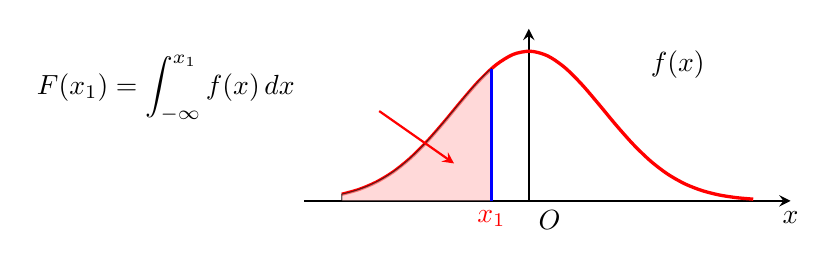
\begin{tikzpicture}[scale=0.95]
        % Plot 1: F(x1)
        \draw[->, >=stealth, thick] (-3,0) -- (3.5,0) node[below] {$x$};
        \draw[->, >=stealth, thick] (0,0) -- (0,2.3);
        \node[below right] at (0,0) {$O$};
        \draw[domain=-2.5:3, smooth, variable=\t, red, very thick] 
            plot ({\t}, {2*exp(-0.5*\t*\t)});
        \node[above right] at (1.5,1.5) {$f(x)$};
        \draw[fill=pink, opacity=0.6] 
            (-2.5,0) -- plot[domain=-2.5:-0.5, smooth, variable=\t] ({\t}, {2*exp(-0.5*\t*\t)}) -- (-0.5,0) -- cycle;
        \draw[blue, thick] (-0.5,0) -- (-0.5,{2*exp(-0.5*0.25)});
        \node[below, red] at (-0.5,0) {$x_1$};
        \node[left] at (-3, 1.5) {$F(x_1) = \displaystyle\int_{-\infty}^{x_1} f(x)\,dx$};
        \draw[->, >=stealth, thick, red] (-2,1.2) -- (-1,0.5);
    \end{tikzpicture}
    \hspace{1cm}
    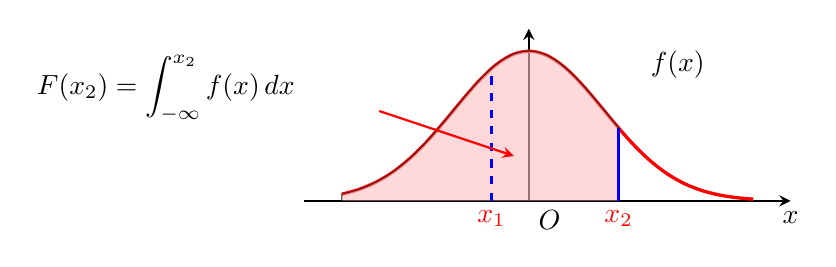
\begin{tikzpicture}[scale=0.95]
        % Plot 2: F(x2)
        \draw[->, >=stealth, thick] (-3,0) -- (3.5,0) node[below] {$x$};
        \draw[->, >=stealth, thick] (0,0) -- (0,2.3);
        \node[below right] at (0,0) {$O$};
        \draw[domain=-2.5:3, smooth, variable=\t, red, very thick] 
            plot ({\t}, {2*exp(-0.5*\t*\t)});
        \node[above right] at (1.5,1.5) {$f(x)$};
        \draw[fill=pink, opacity=0.6] 
            (-2.5,0) -- plot[domain=-2.5:1.2, smooth, variable=\t] ({\t}, {2*exp(-0.5*\t*\t)}) -- (1.2,0) -- cycle;
        \draw[blue, dashed, thick] (-0.5,0) -- (-0.5,{2*exp(-0.5*0.25)});
        \node[below, red] at (-0.5,0) {$x_1$};
        \draw[blue, thick] (1.2,0) -- (1.2,{2*exp(-0.5*1.44)});
        \node[below, red] at (1.2,0) {$x_2$};
        \node[left] at (-3, 1.5) {$F(x_2) = \displaystyle\int_{-\infty}^{x_2} f(x)\,dx$};
        \draw[->, >=stealth, thick, red] (-2,1.2) -- (-0.2,0.6);
    \end{tikzpicture}
    \end{center}
\end{itemize}
\end{nhanxet}

\begin{nhanxet}[Nhận xét 2]
Giả sử BNN rời rạc $X$ nhận các giá trị $x_1 < x_2 < \dots < x_n$, $P(X = x_i) = p_i$ ($i = 1, 2, \dots, n$).
Ta có hàm phân phối của $X$ là:
\[
F(x) = \begin{cases}
0 & \text{khi } x < x_1 \\
p_1 & \text{khi } x_1 \le x < x_2 \\
p_1 + p_2 & \text{khi } x_2 \le x < x_3 \\
\dots\dots\dots\dots\dots\dots\dots\dots\dots\dots\dots\dots \\
p_1 + p_2 + \dots + p_{n-1} & \text{khi } x_{n-1} \le x < x_n \\
1 & \text{khi } x_n \le x.
\end{cases}
\]

\paragraph{Chứng minh:}
\begin{itemize}
    \item $x < x_1$: $F(x) = P(X \le x) = P(X < x_1) = P(\emptyset) = 0$.
    \item $x_1 \le x < x_2$: $F(x) = P(X < x_2) = P(X = x_1) = p_1$.
    \item $x_2 \le x < x_3$: $F(x) = P(X < x_3) = P(X = x_1) + P(X = x_2) = p_1 + p_2$.
    \item[\dots] \dotfill
    \item $x_n \le x$: $F(x) = P(X \le x_n) = P(X = x_1) + \dots + P(X = x_n) = p_1 + \dots + p_n = 1$.
\end{itemize}
\end{nhanxet}

\paragraph{Quy ước.} Nếu BNN $X$ liên tục thì miền xác định của $F(x)$ được lấy theo hàm mật độ $f(x)$.

\begin{itemize}
    \item Giả sử BNN liên tục $X$ có hàm mật độ:
    \[
    f(x) = \begin{cases}
    \varphi(x), & x \in [a; b] \\
    0, & x \notin [a; b].
    \end{cases}
    \]
    Ta có hàm phân phối của $X$ là:
    \[
    F(x) = \begin{cases}
    0 & \text{khi } x < a \\
    \displaystyle\int_a^x \varphi(t)\,dt & \text{khi } a \le x \le b \\
    1 & \text{khi } b < x.
    \end{cases}
    \]

    \item Giả sử BNN liên tục $X$ có hàm mật độ:
    \[
    f(x) = \begin{cases}
    0, & x < a \\
    \varphi(x), & x \ge a.
    \end{cases}
    \]
    Ta có hàm phân phối của $X$ là:
    \[
    F(x) = \begin{cases}
    0 & \text{khi } x < a \\
    \displaystyle\int_a^x \varphi(t)\,dt & \text{khi } x \ge a.
    \end{cases}
    \]

    \item Giả sử BNN liên tục $X$ có hàm mật độ:
    \[
    f(x) = \begin{cases}
    \varphi(x), & x \le a \\
    0, & x > a.
    \end{cases}
    \]
    Ta có hàm phân phối của $X$ là:
    \[
    F(x) = \begin{cases}
    \displaystyle\int_{-\infty}^x \varphi(t)\,dt & \text{khi } x \le a \\
    1 & \text{khi } x > a.
    \end{cases}
    \]
\end{itemize}

\begin{vidu}[VD 1]
Cho BNN $X$ có bảng phân phối xác suất là:
\begin{center}
\begin{tabular}{|c|c|c|c|c|}
\hline
$X$ & $-2$ & $1$ & $3$ & $4$ \\
\hline
$P$ & $0{,}1$ & $0{,}2$ & $0{,}2$ & $0{,}5$ \\
\hline
\end{tabular}
\end{center}
Hãy lập hàm phân phối của $X$ và vẽ đồ thị của $F(x)$?

\paragraph{Giải.} Hàm phân phối của $X$ là:
\[
F(x) = \begin{cases}
0 & \text{khi } x < -2 \\
0{,}1 & \text{khi } -2 \le x < 1 \\
0{,}3 & \text{khi } 1 \le x < 3 \\
0{,}5 & \text{khi } 3 \le x < 4 \\
1 & \text{khi } 4 \le x.
\end{cases}
\]

\textbf{Đồ thị của $F(x)$:}
\begin{center}
\begin{tikzpicture}[scale=1.1]
    \draw[->, >=stealth, thick] (-3.5,0) -- (6,0) node[below] {$x$};
    \draw[->, >=stealth, thick] (0,0) -- (0,3.5) node[right] {$F(x)$};
    \node[below left] at (0,0) {$O$};
    
    % y ticks
    \node[left] at (0,0.5) {$0{,}1$};
    \node[left] at (0,1.0) {$0{,}3$};
    \node[left] at (0,1.5) {$0{,}5$};
    \node[left] at (0,2.5) {$1$};
    
    % x ticks
    \node[below] at (-2,0) {$-2$};
    \node[below] at (1,0) {$1$};
    \node[below] at (3,0) {$3$};
    \node[below] at (4,0) {$4$};

    % Step lines
    % x < -2 : F(x) = 0
    \draw[->, >=stealth, red, very thick] (-2,0) -- (-3.5,0);
    
    % -2 <= x < 1 : F(x) = 0.1
    \filldraw[red] (-2,0.5) circle (1.5pt);
    \draw[red, very thick] (-2,0.5) -- (1,0.5);
    \draw[blue, dotted, thick] (1,0) -- (1,0.5);
    
    % 1 <= x < 3 : F(x) = 0.3
    \filldraw[red] (1,1.0) circle (1.5pt);
    \draw[red, very thick] (1,1.0) -- (3,1.0);
    \draw[blue, dotted, thick] (3,0) -- (3,1.5);
    
    % 3 <= x < 4 : F(x) = 0.5
    \filldraw[red] (3,1.5) circle (1.5pt);
    \draw[red, very thick] (3,1.5) -- (4,1.5);
    \draw[blue, dotted, thick] (4,0) -- (4,2.5);
    
    % x >= 4 : F(x) = 1
    \filldraw[red] (4,2.5) circle (1.5pt);
    \draw[->, >=stealth, red, very thick] (4,2.5) -- (5.5,2.5);
\end{tikzpicture}
\end{center}
\end{vidu}

\begin{vidu}[VD 2]
Cho BNN $X$ có hàm mật độ là:
\[
f(x) = \begin{cases}
0, & x \notin [0; 1] \\
3x^2, & x \in [0; 1].
\end{cases}
\]
Tìm hàm phân phối của $X$ và vẽ đồ thị của $F(x)$?

\paragraph{Giải.} Hàm phân phối của $X$ là:
\[
F(x) = \begin{cases}
0, & x < 0 \\
\displaystyle\int_0^x 3t^2\,dt, & 0 \le x \le 1 \\
1, & 1 < x
\end{cases}
\quad = \quad
\begin{cases}
0, & x < 0 \\
x^3, & 0 \le x \le 1 \\
1, & 1 < x.
\end{cases}
\]

\textbf{Đồ thị của $F(x)$:}
\begin{center}
\begin{tikzpicture}[scale=1.5]
    \draw[->, >=stealth, thick] (-2,0) -- (3.5,0) node[below] {$x$};
    \draw[->, >=stealth, thick] (0,0) -- (0,2.3) node[right] {$F(x)$};
    \node[below left] at (0,0) {$O$};
    
    \node[left] at (0,1.5) {$1$};
    \node[below] at (1.5,0) {$1$};

    % Graph
    \draw[red, very thick] (-2,0) -- (0,0);
    \filldraw[red] (0,0) circle (1.2pt);
    \draw[domain=0:1.5, smooth, variable=\x, red, very thick] 
        plot ({\x}, {1.5*(\x/1.5)*(\x/1.5)*(\x/1.5)});
    \node[above left] at (1.1,0.8) {$x^3$};
    \filldraw[red] (1.5,1.5) circle (1.2pt);
    \draw[dashed, thick] (1.5,0) -- (1.5,1.5);
    \draw[red, very thick] (1.5,1.5) -- (3.2,1.5);
\end{tikzpicture}
\end{center}
\end{vidu}

\begin{vidu}[VD 3]
Cho BNN $X$ có hàm mật độ là:
\[
f(x) = \begin{cases}
0, & x < 100 \\
\dfrac{100}{x^2}, & x \ge 100.
\end{cases}
\]
Tìm hàm phân phối $F(x)$ của $X$?

\paragraph{Giải.} Hàm phân phối $F(x)$ của $X$ là:
\[
F(x) = \begin{cases}
0, & x < 100 \\
100 \displaystyle\int_{100}^x \frac{dt}{t^2}, & x \ge 100
\end{cases}
\quad = \quad
\begin{cases}
0, & x < 100 \\
\dfrac{x - 100}{x}, & x \ge 100.
\end{cases}
\]
\end{vidu}

\subsection{Tính chất của hàm phân phối xác suất}

\begin{enumerate}[label=\arabic*)]
    \item Hàm $F(x)$ xác định với mọi $x \in \mathbb{R}$.
    \item $0 \le F(x) \le 1, \forall x \in \mathbb{R}$; $F(-\infty) = 0$; $F(+\infty) = 1$.
    \item $F(x)$ không giảm và liên tục phải tại mọi $x \in \mathbb{R}$.\\
    Đặc biệt, với $X$ liên tục thì $F(x)$ liên tục $\forall x \in \mathbb{R}$.
    \item $P(a < X \le b) = F(b) - F(a)$.
\end{enumerate}

\paragraph{Đặc biệt:}
\begin{itemize}
    \item Nếu $X$ là BNN rời rạc thì:
    \[
    p_i = F(x_{i+1}) - F(x_i), \quad \forall i.
    \]
    \item Nếu $X$ là BNN liên tục thì:
    \[
    P(a \le X \le b) = P(a \le X < b) = P(a < X \le b) = P(a < X < b) = F(b) - F(a).
    \]
    \item Nếu $X$ là BNN liên tục có hàm mật độ $f(x)$ thì:
    \[
    F'(x) = f(x).
    \]
\end{itemize}

\begin{vidu}[VD 4]
Tính xác suất $P(X \ge 400)$ trong VD 3?

\paragraph{Giải.}
\[
P(X \ge 400) = P(400 \le X < +\infty) = F(+\infty) - F(400) = 1 - \frac{3}{4} = \frac{1}{4}.
\]
\end{vidu}

\begin{vidu}[VD 6]
Cho BNN $X$ có hàm phân phối xác suất:
\[
F(x) = \begin{cases}
0, & x \le -2 \\
ax^3 + 2b, & x \in (-2; 3] \\
1, & x > 3.
\end{cases}
\]
\begin{enumerate}[label=\arabic*)]
    \item Tìm các hằng số $a$ và $b$?
    \item Tính $P(\sqrt{2} < Y \le \sqrt{5})$ với $Y = \sqrt{X^2 + 1}$.
\end{enumerate}

\paragraph{Giải.}
\begin{enumerate}[label=\arabic*)]
    \item Do $F(x)$ liên tục tại mọi $x \in \mathbb{R}$, nên:
    \begin{align*}
    \lim_{x \to -2^+} F(x) = F(-2) &\Rightarrow -8a + 2b = 0 \quad (1), \\
    \lim_{x \to 3^+} F(x) = F(3) &\Rightarrow 27a + 2b = 1 \quad (2).
    \end{align*}
    Từ (1) và (2) ta có: $a = \dfrac{1}{35}$ và $b = \dfrac{4}{35}$.

    \item Ta có:
    \begin{align*}
    P(\sqrt{2} < Y \le \sqrt{5}) &= P\left(\sqrt{2} < \sqrt{X^2 + 1} \le \sqrt{5}\right) \\
    &= P(-2 \le X < -1) + P(1 < X \le 2) \\
    &= F(-1) - F(-2) + F(2) - F(1) = \frac{14}{35}.
    \end{align*}
\end{enumerate}
\end{vidu}

\section{Tham số đặc trưng của biến ngẫu nhiên}

Những thông tin cô đọng phản ánh từng phần về biến ngẫu nhiên giúp ta so sánh giữa các đại lượng với nhau được gọi là các đặc trưng số. Có 3 loại đặc trưng số là:
\begin{itemize}
    \item Các đặc trưng số cho xu hướng trung tâm của BNN: Trung vị, Mode, Kỳ vọng,\dots
    \item Các đặc trưng số cho độ phân tán của BNN: Phương sai, Độ lệch chuẩn,\dots
    \item Các đặc trưng số cho dạng phân phối xác suất.
\end{itemize}

\subsection{Mode}
Mode của biến ngẫu nhiên $X$, ký hiệu $\operatorname{Mod} X$, là giá trị $x_0 \in X$ thỏa:
\begin{itemize}
    \item $P(X = x_0)$ đạt cực đại ($\max$) nếu $X$ là rời rạc, và
    \item $f(x_0)$ đạt cực đại ($\max$) nếu $X$ liên tục có hàm mật độ $f(x)$.
\end{itemize}

\begin{chuy}
\begin{itemize}
    \item $\operatorname{Mod} X$ còn được gọi là giá trị tin chắc nhất của $X$.
    \item Biến ngẫu nhiên $X$ có thể có nhiều $\operatorname{Mod} X$.
\end{itemize}
\end{chuy}

\begin{vidu}[VD 1]
Cho BNN $X$ có bảng phân phối xác suất:
\begin{center}
\begin{tabular}{|c|c|c|c|c|c|c|}
\hline
$X$ & $0$ & $1$ & $2$ & $4$ & $5$ & $8$ \\
\hline
$P$ & $0{,}10$ & $0{,}20$ & $0{,}30$ & $0{,}05$ & $0{,}25$ & $0{,}10$ \\
\hline
\end{tabular}
\end{center}
Giá trị có xác suất lớn nhất là $P(X = 2) = 0{,}30 \Rightarrow \operatorname{Mod} X = 2$.
\end{vidu}

\begin{vidu}[VD 2]
Tìm $\operatorname{Mod} X$, biết $X$ có bảng phân phối xác suất:
\begin{center}
\begin{tabular}{|c|c|c|c|c|c|}
\hline
$X$ & $1$ & $2$ & $4$ & $5$ & $8$ \\
\hline
$P$ & $1 - 3p$ & $0{,}18$ & $0{,}07$ & $0{,}25$ & $p$ \\
\hline
\end{tabular}
\end{center}

\paragraph{Giải.} Ta có:
\[
1 - 3p + 0{,}18 + 0{,}07 + 0{,}25 + p = 1 \Rightarrow p = 0{,}25.
\]
Khi đó $P(X = 1) = 1 - 3(0{,}25) = 0{,}25$; $P(X = 5) = 0{,}25$; $P(X = 8) = 0{,}25$.\\
Vậy $\operatorname{Mod} X = 1; 5; 8$.
\end{vidu}

\begin{vidu}[VD 3]
Tìm $\operatorname{Mod} X$, biết $X$ có hàm mật độ xác suất:
\[
f(x) = \begin{cases}
\dfrac{3}{64} x^2 (4 - x), & x \in [0; 4] \\
0, & x \notin [0; 4].
\end{cases}
\]

\paragraph{Giải.} Với $x \in [0; 4]$, ta có:
\[
f'(x) = 0 \Leftrightarrow x = 0, \quad x = \frac{8}{3}.
\]
\[
f(0) = f(4) = 0, \quad f\left(\frac{8}{3}\right) = \frac{4}{9}.
\]
\[
\Rightarrow \max_{\mathbb{R}} f(x) = f\left(\frac{8}{3}\right) = \frac{4}{9}. \quad \text{Vậy } \operatorname{Mod} X = \frac{8}{3}.
\]
\end{vidu}

\subsection{Kỳ vọng}

\subsubsection{Định nghĩa}
Kỳ vọng (\textit{Expectation}) của biến ngẫu nhiên $X$, ký hiệu $EX$ hay $M(X)$, là một số thực được xác định như sau:
\begin{itemize}
    \item Nếu $X$ là rời rạc với xác suất $P(X = x_i) = p_i$ thì:
    \[
    EX = \sum_i x_i p_i.
    \]
    \item Nếu $X$ là liên tục có hàm mật độ $f(x)$ thì:
    \[
    EX = \int_{-\infty}^{+\infty} x f(x)\,dx.
    \]
\end{itemize}

\paragraph{Đặc biệt.} Nếu biến ngẫu nhiên rời rạc $X = \{x_1; x_2; \dots; x_n\}$ với xác suất tương ứng là $p_1, p_2, \dots, p_n$ thì:
\[
EX = x_1 p_1 + x_2 p_2 + \dots + x_n p_n.
\]

\begin{vidu}[VD 4]
Cho BNN $X$ có bảng phân phối xác suất:
\begin{center}
\begin{tabular}{|c|c|c|c|c|}
\hline
$X$ & $-1$ & $0$ & $2$ & $3$ \\
\hline
$P$ & $0{,}1$ & $0{,}2$ & $0{,}4$ & $0{,}3$ \\
\hline
\end{tabular}
\end{center}
Tính kỳ vọng của $X$?

\paragraph{Giải.} Ta có:
\[
EX = -1 \times 0{,}1 + 0 \times 0{,}2 + 2 \times 0{,}4 + 3 \times 0{,}3 = 1{,}6.
\]
\end{vidu}

\begin{vidu}[VD 6]
Tìm kỳ vọng của BNN $X$ có hàm mật độ:
\[
f(x) = \begin{cases}
\dfrac{3}{4}(x^2 + 2x), & x \in [0; 1] \\
0, & x \notin [0; 1].
\end{cases}
\]

\paragraph{Giải.}
\[
EX = \int_{-\infty}^{+\infty} x f(x)\,dx = \int_0^1 x \cdot \frac{3}{4}(x^2 + 2x)\,dx = \frac{3}{4} \int_0^1 (x^3 + 2x^2)\,dx = \frac{3}{4} \left.\left(\frac{x^4}{4} + \frac{2x^3}{3}\right)\right|_0^1 = \frac{11}{16}.
\]
\end{vidu}

\begin{chuy}
\begin{itemize}
    \item Nếu $X$ là BNN liên tục trên $[a; b]$ thì $EX \in [a; b]$.
    \item Nếu $X = \{x_1, \dots, x_n\}$ thì $EX \in [\min\{x_1, \dots, x_n\}; \max\{x_1, \dots, x_n\}]$.
\end{itemize}
\end{chuy}

\subsubsection{Tính chất của Kỳ vọng}
\begin{enumerate}[label=\arabic*)]
    \item $EC = C$, $C \in \mathbb{R}$.
    \item $E(CX) = C \cdot EX$, $C \in \mathbb{R}$.
    \item $E(X \pm Y) = EX \pm EY$.
    \item $E(X \cdot Y) = EX \cdot EY$ nếu $X, Y$ độc lập.
\end{enumerate}

\paragraph{Bài tập về nhà.} Cho hai biến ngẫu nhiên $X, Y$ độc lập có bảng phân phối xác suất:
\begin{center}
\begin{tabular}{|c|c|c|c|}
\hline
$X$ & $-1$ & $1$ & $3$ \\
\hline
$P$ & $0{,}3$ & $0{,}1$ & $0{,}6$ \\
\hline
\end{tabular}
\qquad
\begin{tabular}{|c|c|c|}
\hline
$Y$ & $-1$ & $2$ \\
\hline
$P$ & $0{,}6$ & $0{,}4$ \\
\hline
\end{tabular}
\end{center}
Tính $E(X^2 \cdot Y - 3XY + 5Y + 7)$.

\subsubsection{Ý nghĩa của Kỳ vọng}
\begin{itemize}
    \item Kỳ vọng của biến ngẫu nhiên $X$ là giá trị trung bình (tính theo xác suất) mà $X$ nhận được, nó phản ánh giá trị trung tâm phân phối xác suất của $X$.
    \item Trong thực tế sản xuất hay kinh doanh, khi cần chọn phương án cho năng suất hay lợi nhuận cao, người ta thường chọn phương án sao cho kỳ vọng năng suất hay kỳ vọng lợi nhuận cao.
\end{itemize}

\begin{vidu}[VD 9]
Một thống kê cho biết tỉ lệ tai nạn xe máy ở thành phố H là 0,001. Công ty bảo hiểm A đề nghị bán loại bảo hiểm tai nạn xe máy cho ông B ở thành phố H trong 1 năm với số tiền chi trả là 10 (triệu đồng), phí bảo hiểm là 0,1 (triệu đồng). Hỏi trung bình công ty A lãi bao nhiêu khi bán bảo hiểm cho ông B?

\paragraph{Giải.} Gọi $X$ (triệu đồng) là tiền lãi của công ty A sau khi bán bảo hiểm cho ông B.
\begin{itemize}
    \item Khi ông B không bị tai nạn thì: $X = 0{,}1$ và xác suất $p = 0{,}999$.
    \item Khi ông B bị tai nạn thì: $X = 0{,}1 - 10 = -9{,}9$; $p = 0{,}001$.
\end{itemize}
Vậy trung bình tiền lãi của công ty A là:
\[
EX = 0{,}1 \times 0{,}999 - 9{,}9 \times 0{,}001 = 0{,}09 \text{ (triệu đồng)}.
\]
\end{vidu}

\subsubsection{Kỳ vọng của hàm của biến ngẫu nhiên}
Giả sử $Y = \varphi(X)$ là hàm của biến ngẫu nhiên $X$.
\begin{itemize}
    \item Nếu $X$ là biến ngẫu nhiên rời rạc thì:
    \[
    EY = \sum_i y_i p_i = \sum_i \varphi(x_i) p_i.
    \]
    \item Nếu $X$ là biến ngẫu nhiên liên tục thì:
    \[
    EY = \int_{-\infty}^{+\infty} y f(x)\,dx = \int_{-\infty}^{+\infty} \varphi(x) f(x)\,dx.
    \]
\end{itemize}

\begin{chuy}
Khi biến ngẫu nhiên $X$ là rời rạc thì ta nên lập bảng phân phối xác suất của $Y$, rồi tính $EY$.
\end{chuy}

\begin{vidu}[VD 13]
Cho BNN $X$ có bảng phân phối xác suất:
\begin{center}
\begin{tabular}{|c|c|c|c|c|}
\hline
$X$ & $-1$ & $0$ & $1$ & $2$ \\
\hline
$P$ & $0{,}1$ & $0{,}3$ & $0{,}35$ & $0{,}25$ \\
\hline
\end{tabular}
\end{center}
Tính $EY$ với $Y = X^2 - 3$?

\paragraph{Giải.} Ta có bảng phân phối xác suất của $Y$ là:
\begin{center}
\begin{tabular}{|c|c|c|c|}
\hline
$Y$ & $-3$ & $-2$ & $1$ \\
\hline
$P$ & $0{,}3$ & $0{,}45$ & $0{,}25$ \\
\hline
\end{tabular}
\end{center}
Vậy:
\[
EY = -3 \cdot 0{,}3 - 2 \cdot 0{,}45 + 1 \cdot 0{,}25 = -1{,}55.
\]
\end{vidu}

\begin{vidu}[VD 14]
Cho BNN $X$ có hàm mật độ xác suất:
\[
f(x) = \begin{cases}
\dfrac{2}{x^2}, & x \in [1; 2] \\
0, & x \notin [1; 2].
\end{cases}
\]
Tính $EY$ với $Y = X^5 - \dfrac{2}{X}$?

\paragraph{Giải.} Áp dụng công thức, ta có:
\[
EY = \int_{-\infty}^{+\infty} y f(x)\,dx = \int_1^2 \left(x^5 - \frac{2}{x}\right) \cdot \frac{2}{x^2}\,dx = \left.\left(\frac{x^4}{2} + \frac{2}{x^2}\right)\right|_1^2 = 6.
\]
\end{vidu}

\subsection{Phương sai}

\subsubsection{Định nghĩa}
Phương sai (\textit{Variance} hay \textit{Dispersion}) của biến ngẫu nhiên $X$, ký hiệu $\operatorname{Var} X$ hay $D(X)$, là một số thực không âm được xác định bởi:
\[
\operatorname{Var} X = E(X - EX)^2 = E(X^2) - (EX)^2.
\]
Ta có:
\begin{align*}
\operatorname{Var} X &= E\left[(X - EX)^2\right] \\
&= E\left[X^2 - 2X \cdot EX + (EX)^2\right] \\
&= E(X^2) - 2 \cdot EX \cdot EX + (EX)^2 \\
&= E(X^2) - (EX)^2.
\end{align*}

\begin{itemize}
    \item Nếu BNN $X$ là rời rạc và $P(X = x_i) = p_i$ thì:
    \[
    \operatorname{Var} X = \sum_i x_i^2 p_i - \left(\sum_i x_i p_i\right)^2.
    \]
    \item Nếu BNN $X$ là liên tục và có hàm mật độ $f(x)$ thì:
    \[
    \operatorname{Var} X = \int_{-\infty}^{+\infty} x^2 f(x)\,dx - \left(\int_{-\infty}^{+\infty} x f(x)\,dx\right)^2.
    \]
\end{itemize}

\begin{vidu}[VD 15]
Cho BNN $X$ có bảng phân phối xác suất:
\begin{center}
\begin{tabular}{|c|c|c|c|}
\hline
$X$ & $1$ & $2$ & $3$ \\
\hline
$P$ & $0{,}2$ & $0{,}7$ & $0{,}1$ \\
\hline
\end{tabular}
\end{center}
Ta có:
\[
\operatorname{Var} X = (1^2 \cdot 0{,}2 + 2^2 \cdot 0{,}7 + 3^2 \cdot 0{,}1) - (1 \cdot 0{,}2 + 2 \cdot 0{,}7 + 3 \cdot 0{,}1)^2 = 0{,}29.
\]
\end{vidu}

\begin{vidu}[VD 16]
Tính phương sai của $X$, biết hàm mật độ:
\[
f(x) = \begin{cases}
\dfrac{3}{4}(x^2 + 2x), & x \in [0; 1] \\
0, & x \notin [0; 1].
\end{cases}
\]

\paragraph{Giải.} Áp dụng công thức, ta có:
\begin{align*}
\operatorname{Var} X &= \int_0^1 x^2 \cdot \frac{3}{4}(x^2 + 2x)\,dx - \left[\int_0^1 x \cdot \frac{3}{4}(x^2 + 2x)\,dx\right]^2 \\
&= \frac{3}{4} \left.\left(\frac{x^5}{5} + \frac{x^4}{2}\right)\right|_0^1 - \left[\frac{3}{4} \left.\left(\frac{x^4}{4} + \frac{2x^3}{3}\right)\right|_0^1\right]^2 = \frac{67}{1280}.
\end{align*}
\end{vidu}

\begin{vidu}[VD 17]
Cho BNN $X$ có hàm mật độ xác suất:
\[
f(x) = \begin{cases}
\dfrac{3}{4}(1 - x^2), & |x| \le 1 \\
0, & |x| > 1.
\end{cases}
\]
Tính phương sai của $Y$, cho biết $Y = 2X^2$.

\paragraph{Giải.}
\begin{align*}
\operatorname{Var} Y &= \int_{-1}^1 y^2 \cdot f(x)\,dx - \left[\int_{-1}^1 y \cdot f(x)\,dx\right]^2 \\
&= \int_{-1}^1 (2x^2)^2 \cdot \frac{3}{4}(1 - x^2)\,dx - \left[\int_{-1}^1 2x^2 \cdot \frac{3}{4}(1 - x^2)\,dx\right]^2 \\
&= 3\left.\left(\frac{x^5}{5} - \frac{x^7}{7}\right)\right|_{-1}^1 - \left[\frac{3}{2}\left.\left(\frac{x^3}{3} - \frac{x^5}{5}\right)\right|_{-1}^1\right]^2 = \frac{32}{175}.
\end{align*}
\end{vidu}

\subsubsection{Tính chất của Phương sai}
\begin{enumerate}[label=\arabic*)]
    \item $\operatorname{Var} C = 0$, $C \in \mathbb{R}$;
    \item $\operatorname{Var}(CX) = C^2 \operatorname{Var} X$;
    \item $\operatorname{Var}(X \pm Y) = \operatorname{Var} X + \operatorname{Var} Y$ nếu $X$ và $Y$ độc lập.
\end{enumerate}

\subsubsection{Ý nghĩa của Phương sai}
\begin{itemize}
    \item $(X - EX)^2$ là bình phương sai biệt giữa giá trị của $X$ so với trung bình của nó. Và phương sai là trung bình của sai biệt này, nên phương sai cho ta hình ảnh về \textbf{sự phân tán} của các số liệu: phương sai càng nhỏ thì số liệu càng tập trung xung quanh trung bình của chúng.
    \item Trong kỹ thuật, phương sai đặc trưng cho độ sai số của thiết bị. Trong kinh doanh, phương sai đặc trưng cho độ rủi ro đầu tư.
    \item Do đơn vị đo của $\operatorname{Var} X$ bằng bình phương đơn vị đo của $X$ nên để so sánh được với các đặc trưng khác, người ta đưa vào khái niệm \textbf{độ lệch tiêu chuẩn} (\textit{standard deviation}) là:
    \[
    \sigma = \sqrt{\operatorname{Var} X}.
    \]
\end{itemize}

\begin{vidu}[VD 18]
Năng suất (sản phẩm/phút) của hai máy tương ứng là các BNN $X$ và $Y$, có bảng phân phối xác suất:
\begin{center}
\begin{tabular}{|c|c|c|c|c|}
\hline
$X$ & $1$ & $2$ & $3$ & $4$ \\
\hline
$P$ & $0{,}3$ & $0{,}1$ & $0{,}5$ & $0{,}1$ \\
\hline
\end{tabular}
\qquad
\begin{tabular}{|c|c|c|c|c|}
\hline
$Y$ & $2$ & $3$ & $4$ & $5$ \\
\hline
$P$ & $0{,}1$ & $0{,}4$ & $0{,}4$ & $0{,}1$ \\
\hline
\end{tabular}
\end{center}
Từ bảng phân phối xác suất, ta tính được:
\[
EX = 2{,}4; \quad \operatorname{Var} X = 1{,}04; \quad EY = 3{,}5; \quad \operatorname{Var} Y = 0{,}65.
\]
Vì $EX < EY$, $\operatorname{Var} X > \operatorname{Var} Y$ nên nếu phải chọn mua một trong hai loại máy này thì ta chọn mua máy $Y$.
\end{vidu}

\begin{chuy}
Trong trường hợp:
\[
\begin{cases}
EX < EY \\
\operatorname{Var} X < \operatorname{Var} Y
\end{cases}
\quad \text{hay} \quad
\begin{cases}
EX > EY \\
\operatorname{Var} X > \operatorname{Var} Y
\end{cases}
\]
thì ta không thể so sánh được. Để giải quyết vấn đề này, trong thực tế người ta dùng \textbf{tỉ số tương đối} $\dfrac{\sigma}{\mu} \cdot 100\%$ ($\mu$ là trung bình) để so sánh sự ổn định của các BNN $X$ và $Y$. Tỉ số tương đối \textbf{càng nhỏ} thì \textbf{độ ổn định càng cao}.
\end{chuy}

\begin{vidu}[VD 19]
Điểm thi hết môn XSTK của lớp A và B tương ứng là các BNN $X$ và $Y$. Người ta tính được:
\[
EX = 6{,}25; \quad \operatorname{Var} X = 1{,}25; \quad EY = 5{,}75; \quad \operatorname{Var} Y = 0{,}75.
\]
Ta có:
\[
\frac{\sigma_x}{EX} \cdot 100\% = 17{,}89\%; \qquad \frac{\sigma_y}{EY} \cdot 100\% = 15{,}06\%.
\]
Vậy lớp B học đều (ổn định) hơn lớp A.
\end{vidu}

\subsection{Trung vị (tham khảo)}
Trung vị (\textit{median}) của BNN $X$, ký hiệu $\operatorname{Med} X$, là số thực $m$ thỏa:
\[
P(X \le m) = P(X \ge m).
\]

\begin{vidu}[VD 1]
Cho BNN $X$ có bảng phân phối xác suất:
\begin{center}
\begin{tabular}{|c|c|c|c|c|}
\hline
$X$ & $0$ & $1$ & $2$ & $3$ \\
\hline
$P$ & $0{,}125$ & $0{,}375$ & $0{,}375$ & $0{,}125$ \\
\hline
\end{tabular}
\end{center}
Ta có: $\operatorname{Med} X = m$ thỏa $1 < m < 2$.
\end{vidu}

\begin{vidu}[VD 2]
Cho BNN $X$ có hàm mật độ:
\[
f(x) = \frac{2}{9} \begin{cases}
3x - x^2, & x \in [0; 3] \\
0, & x \notin [0; 3].
\end{cases}
\]
Ta có: $P(X \le m) = P(X \ge m) \Rightarrow \operatorname{Med} X = m \in [0; 3]$
\[
\Rightarrow \frac{1}{2} = \frac{2}{9} \int_0^m (3x - x^2)\,dx \Rightarrow m = \frac{3}{2} \in [0; 3].
\]
\end{vidu}

\paragraph{Minh họa hình học các tham số đặc trưng:}
\begin{center}
\begin{tikzpicture}[scale=0.85]
    % Mode
    \begin{scope}[shift={(0,3.5)}]
        \draw[fill=gray!40] (-1.8,0) -- plot[domain=-1.8:2.5, smooth] ({\x}, {2.2*exp(-0.5*(\x+0.8)*(\x+0.8))}) -- (2.5,0) -- cycle;
        \draw[thick] (-2,0) -- (3,0);
        \draw[red, very thick] (-0.8,0) -- (-0.8,2.2);
        \draw[orange, thick] (-1.1,2.2) -- (-0.5,2.2);
        \node[below] at (-0.8,-0.2) {\textbf{mode}};
    \end{scope}

    % Mean
    \begin{scope}[shift={(0,0)}]
        \draw[fill=gray!40] (-1.8,0) -- plot[domain=-1.8:2.5, smooth] ({\x}, {2.2*exp(-0.5*(\x+0.8)*(\x+0.8))}) -- (2.5,0) -- cycle;
        \draw[thick] (-2,0) -- (3,0);
        \fill[blue] (-0.3,-0.2) -- (-0.1,0) -- (-0.5,0) -- cycle;
        \node[below] at (-0.3,-0.3) {\textbf{mean}};
    \end{scope}

    % Median
    \begin{scope}[shift={(6,1.5)}]
        \draw[fill=yellow!40] (-1.8,0) -- plot[domain=-1.8:-0.3, smooth] ({\x}, {2.2*exp(-0.5*(\x+0.8)*(\x+0.8))}) -- (-0.3,0) -- cycle;
        \draw[fill=cyan!30] (-0.3,0) -- plot[domain=-0.3:2.5, smooth] ({\x}, {2.2*exp(-0.5*(\x+0.8)*(\x+0.8))}) -- (2.5,0) -- cycle;
        \draw[thick] (-2,0) -- (3,0);
        \draw[green!60!black, very thick] (-0.3,0) -- (-0.3,1.95);
        \node at (-1.0,0.6) {50\%};
        \node at (0.4,0.6) {50\%};
        \node[below] at (-0.3,-0.2) {\textbf{median}};
    \end{scope}

    % Variance
    \begin{scope}[shift={(3,-3.8)}]
        \draw[->, >=stealth, thick] (-3,0) -- (3.5,0);
        \draw[thick] (0,0) -- (0,3);
        \draw[domain=-2.2:2.2, smooth, very thick] plot ({\x}, {2.6*exp(-2*\x*\x)});
        \draw[domain=-2.8:2.8, smooth, thick] plot ({\x}, {1.3*exp(-0.5*\x*\x)});
        \node[below] at (0,0) {$\mu$};
        \draw[->, >=stealth] (1.5,1.8) -- (0.5,1.2);
        \node[right] at (1.5,1.8) {\small Phương sai nhỏ};
        \draw[->, >=stealth] (1.8,0.8) -- (1.1,0.5);
        \node[right] at (1.8,0.8) {\small Phương sai lớn};
    \end{scope}
\end{tikzpicture}
\end{center}

\vspace{1.5em}
\hrule
\vspace{1.5em}

\section{Bài tập}

\begin{enumerate}[label=\textbf{\arabic*.}]
    \item Một xạ thủ có 4 viên đạn, bắn lần lượt từng viên vào một mục tiêu một cách độc lập. Xác suất trúng mục tiêu ở mỗi lần bắn là $0{,}8$. Biết rằng, nếu có 1 viên trúng mục tiêu hoặc hết đạn thì dừng. Gọi $X$ là số viên đạn xạ thủ đã bắn, hãy lập bảng phân phối xác suất của $X$?

    \item Cho BNN $X$ có hàm mật độ:
    \[
    f(x) = \begin{cases}
    \dfrac{3}{28} x^2, & x \in [-1; 3] \\
    0, & x \notin [-1; 3].
    \end{cases}
    \]
    Tìm hàm phân phối $F(x)$ của $X$?

    \item Cho $X$ là ĐLNN liên tục với hàm mật độ:
    \[
    f(x) = \begin{cases}
    kx, & x \in [0, 1] \\
    0, & x \notin [0, 1].
    \end{cases}
    \]
    \begin{enumerate}[label=\arabic*)]
        \item Xác định giá trị $k$.
        \item Tìm hàm phân phối $F(x)$.
        \item Tính các xác suất $P\left(X < \dfrac{1}{2}\right)$ và $P\left(\dfrac{1}{2} < X < \dfrac{3}{4}\right)$.
    \end{enumerate}

    \item Một lô hàng gồm 10 sản phẩm tốt và 2 phế phẩm. Lấy ngẫu nhiên 4 sản phẩm từ lô hàng đó, gọi $X$ là số sản phẩm tốt trong 4 sản phẩm lấy ra. Tìm phân phối xác suất và tính kỳ vọng của $X$?

    \item Cho BNN $X$ có bảng phân phối xác suất:
    \begin{center}
    \begin{tabular}{|c|c|c|c|c|c|}
    \hline
    $X$ & $1$ & $2$ & $4$ & $5$ & $7$ \\
    \hline
    $P$ & $a$ & $0{,}2$ & $b$ & $0{,}2$ & $0{,}1$ \\
    \hline
    \end{tabular}
    \end{center}
    Tìm giá trị của tham số $a$ và $b$ để $EX = 3{,}5$?

    \item Ông $A$ tham gia một trò chơi đỏ, đen như sau: Trong một hộp có 4 bi đỏ và 6 bi đen. Mỗi lần ông $A$ lấy ra 1 bi: nếu là đỏ thì được thưởng 100 (ngàn đồng), nếu là đen thì bị mất 70 (ngàn đồng). Hỏi trung bình mỗi lần lấy bi ông $A$ nhận được bao nhiêu tiền?

    \item Người thợ chép tranh mỗi tuần chép hai bức tranh độc lập $A$ và $B$ với xác suất hỏng tương ứng là $0{,}03$ và $0{,}05$. Nếu thành công thì người thợ sẽ kiếm lời từ bức tranh $A$ là $1{,}3$ triệu đồng và $B$ là $0{,}9$ triệu đồng, nhưng nếu hỏng thì bị lỗ do bức tranh $A$ là $0{,}8$ triệu đồng và do $B$ là $0{,}6$ triệu đồng. Hỏi trung bình người thợ nhận được bao nhiêu tiền chép tranh mỗi tuần?

    \item Cho một kiện hàng có 6 sản phẩm loại 1, 4 sản phẩm loại 2. Chọn ngẫu nhiên có hoàn lại 2 sản phẩm từ kiện hàng này. Gọi $X$ là số sản phẩm loại 1 trong 2 sản phẩm được lấy ra.
    \begin{enumerate}[label=\arabic*)]
        \item Tìm luật phân phối xác suất của $X$.
        \item Tìm kỳ vọng $E(X)$.
        \item Tìm phương sai $\operatorname{Var}(X)$.
    \end{enumerate}

    \item Một doanh nghiệp đầu tư phát triển một loại sản phẩm mới, xác suất thành công là $30\%$. Chi phí đầu tư bỏ ra là 100 nghìn USD. Nếu không thành công thì mất chi phí đầu tư mà không thu về được gì, nhưng nếu thành công thì thu về được 1 triệu USD (trước khi trừ đi chi phí đầu tư). Tính kỳ vọng lợi nhuận từ dự án đầu tư này.

    \item Cho ĐLNN $X$ có hàm mật độ xác suất như sau:
    \[
    f(x) = \begin{cases}
    2e^{-2x}, & x \ge 0 \\
    0, & x < 0.
    \end{cases}
    \]
    Tìm các giá trị:
    \begin{enumerate}[label=\arabic*)]
        \item Kỳ vọng $E(X)$.
        \item Phương sai $\operatorname{Var}(X)$ và độ lệch chuẩn $\sigma$.
        \item $\operatorname{Mod}(X)$.
    \end{enumerate}
\end{enumerate}
